\documentclass[9pt]{beamer}
\usetheme{TUDOplain}
% workaround: provide commands not defiend by all bibtex styles
\providecommand{\btxandlong}{und}
\providecommand{\newblock}{}

% sourcing images
\providecommand{\source}{\\ \footnotesize \tugreen{Source:} \footnotemark}
\providecommand{\sourcefix}[1]{\\ \footnotesize \tugreen{Source:} [#1]}

\renewcommand{\caption}[1]{\\ \footnotesize{\captiongrey{#1}}}

\usepackage[english]{babel}
\usepackage[style=authortitle]{biblatex}
\addbibresource{../bibliography.bib}

% reformat footnotes very plain
\makeatletter
\renewcommand\@makefnmark{%
[\@thefnmark]}
\renewcommand\@makefntext[1]{%
  \noindent\tiny [\@thefnmark] #1}
\makeatother
% command for citing
\providecommand{\fcite}[1]{\footcite{#1}}
%

% basic utils
\usepackage[utf8]{inputenc}
\usepackage{enumerate}
\usepackage{graphicx}
\graphicspath{{../images/}}

\AtBeginSection[]{
  \begin{frame}
  \vfill
  \centering
  \begin{beamercolorbox}[sep=8pt,center,shadow=true,rounded=true]{title}
    \usebeamerfont{title}\insertsectionhead\par%
  \end{beamercolorbox}
  \vfill
  \end{frame}
}

\usepackage{ifthen}
\usepackage{calc}
\usepackage{amsmath,amsfonts,amssymb}
\setbeamertemplate{navigation symbols}{}
%\setbeamertemplate{footline}{}
%\setbeamertemplate{footline}[frame number]{}
\setbeamertemplate{footline}{\small \vspace{-1ex} \vbox{ \insertframenumber /\inserttotalframenumber}}
%\setbeamertemplate{footline}{\fontsize{7pt}{7pt}\selectfont \vspace{-1ex} \vbox{ \insertframenumber /\inserttotalframenumber}}

\author{Matthias Jakobs}
\title{End-to-end Human Activity Recognition framework on Complex Video Datasets}
\date{\today}
\institute[TU Dortmund]{Pattern Recognition In Embedded Systems,\\ Department of Computer Science \\ LS XII, Technische Universität Dortmund}
%
% frame command
\newenvironment{myframe}[1][]{%
\begin{frame}%
\frametitle{#1}
% start footnote numbers with 1
\setcounter{footnote}{0}


}{%
\end{frame}%
}

\begin{document}
\begin{frame}

\titlepage

\end{frame}

\section{Motivation}
\begin{myframe}[Motivation]
  \begin{figure}
    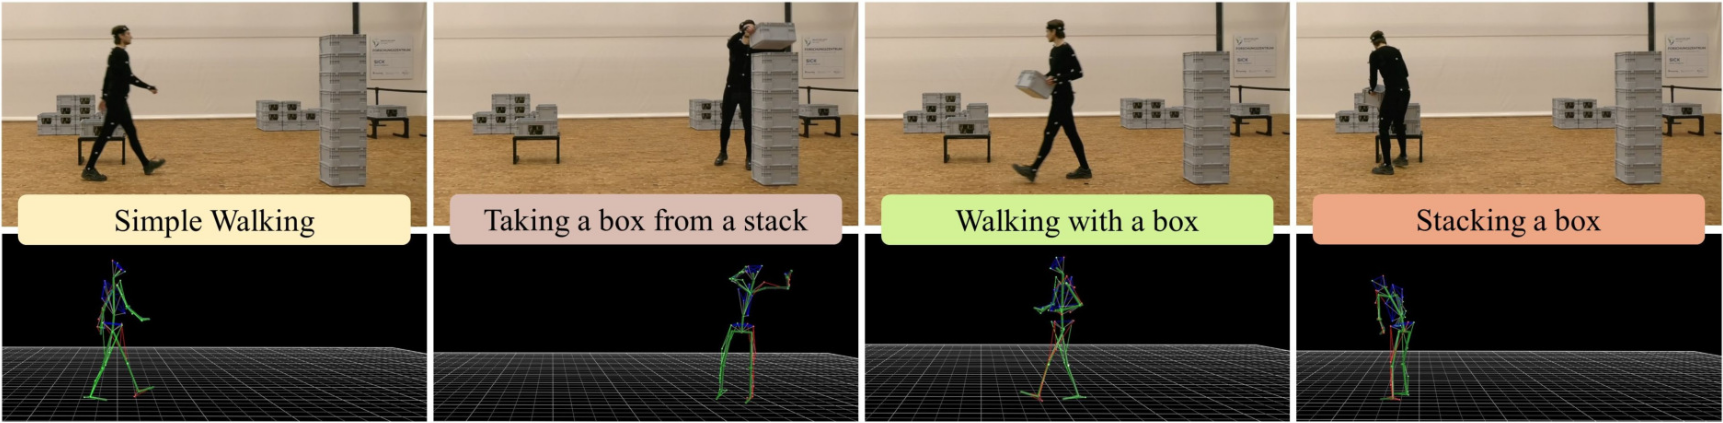
\includegraphics[width=\textwidth]{har-image-skeleton.png}
    \caption{Example of human activities in a warehouse context.}
    \source
  \end{figure}
  \begin{itemize}
      \item Motion capturing costly
      \item Pose estimators become better rapidly
      \item End-to-end training recently proposed
  \end{itemize}
  \footnotetext[1]{\cite{reining_towards_2018}}
\end{myframe}

\tableofcontents

\section{Fundamentals}
\subsection{Human Activity Recognition}

\begin{myframe}[Fundamentals - HAR]
    \begin{columns}
        \begin{column}{.48\textwidth}
            \begin{itemize}
                \item Identify actions performed by humans
                \item Some use-cases:
                    \begin{itemize}
                        \item Video surveillance
                        \item Human-computer interaction
                        \item Warehouse scenario from before
                    \end{itemize}
                \item Multiple sources for detection
                \begin{itemize}
                    \item Inertial Measurement Units (IMUs)
                    \item Images (or video)
                \end{itemize}
            \end{itemize}
        \end{column}
        \begin{column}{.48\textwidth}
            \begin{figure}
                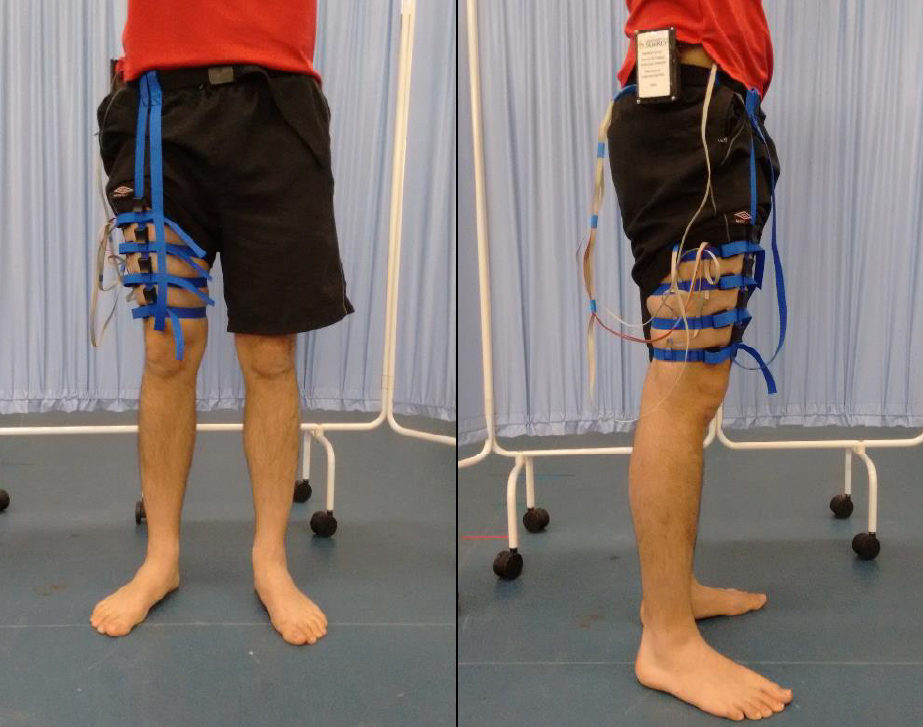
\includegraphics[width=0.99\textwidth]{imu.jpg}
                \caption{Inertial Measurement Units manufactured by Surrey Sensors}
                \source
            \end{figure}
        \end{column}
    \end{columns}
    \footnotetext[1]{\url{http://surreysensors.com/wp-content/uploads/2017/02/IMU.jpg}}
\end{myframe}

\begin{myframe}[Fundamentals - HAR]
    \begin{columns}
        \begin{column}{.48\linewidth}
            \begin{itemize}
                \item High degree of interclass variance
                \item How fine-grained?
                \begin{itemize}
                    \item \textit{Raising left arm} or
                    \item \textit{Waving}
                    \item \textit{attributes} vs. \textit{actions} \footnotemark
                \end{itemize}
            \end{itemize}
        \end{column}
        \begin{column}{.48\linewidth}
            \begin{figure}
                \includegraphics[width=0.99\textwidth]{attributes-actions.png}
                \sourcefix{1}
            \end{figure}
        \end{column}
    \end{columns}
    \footnotetext[1]{\cite{reining_towards_2018}}
\end{myframe}

\subsection{Pose Estimation}

\begin{myframe}[Fundamentals - Pose Estimation]
    \begin{columns}[T]
        \begin{column}{0.45\textwidth}
            \vspace{30px}
            \begin{itemize}
                \item Detect joint locations
                \item Different definitions
                \item Single vs. multi person
                \item 2D and 3D methods
            \end{itemize}
        \end{column}
        \begin{column}{0.55\textwidth}
            \begin{figure}
                \includegraphics[width=.89\textwidth]{pe-singlehumna.png}
                \source
            \end{figure}
        \end{column}
    \end{columns}
    \begin{figure}
        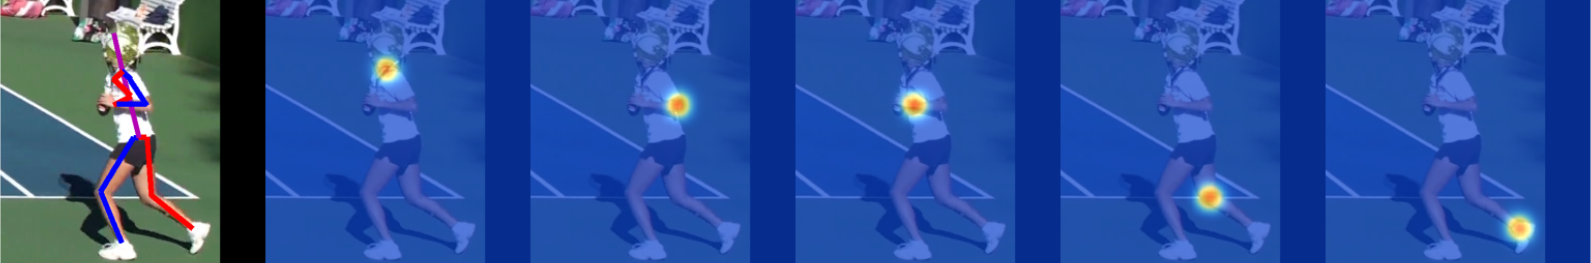
\includegraphics[height=50px]{2dheatmaps.png}
        \source
    \end{figure}
    \footnotetext[1]{\url{https://blog.nanonets.com/content/images/2019/04/Screen-Shot-2019-04-11-at-5.17.56-PM.png}}
    \footnotetext[2]{\cite{newell_stacked_2016}}
\end{myframe}

\begin{myframe}[Fundamentals - Pose Estimation]
    \begin{figure}
        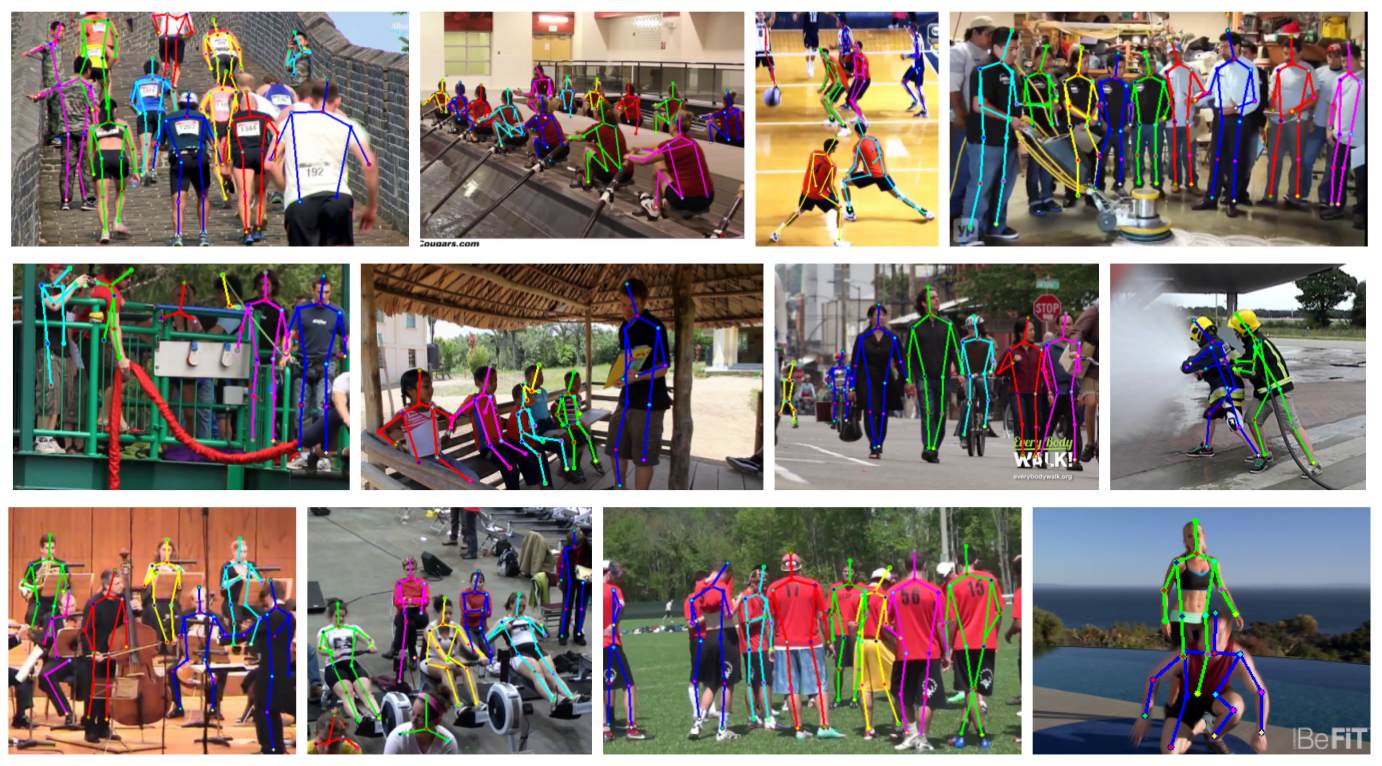
\includegraphics[width=.99\textwidth]{pe-multihuman.png}
        \caption{Example of hard multi-person pose estimation situations.}
        \source
    \end{figure}
    \footnotetext[1]{\url{http://pages.iai.uni-bonn.de/iqbal_umar/multiperson-pose/}}
\end{myframe}

\section{Related Work}
\subsection{Pose Estimation}

\begin{myframe}[Pose Estimation - Shallow Methods]
    \begin{columns}[T]
        \begin{column}{.48\textwidth}
            \begin{itemize}
                \item \textbf{Pictoral Structures for Object Recognition \footnotemark}
              \begin{itemize}
                  \item Based on initial work by \footnotemark
                  \item Binary images (background subtraction)
                  \item \textit{Model each limb}
                  \begin{itemize}
                      \item Approximate each limb as rectangle using $\ell = (x,y,s,\theta)$
                      \item Maximize covered foreground pixels by parts $p(I \lvert \ell,c)$
                  \end{itemize}
                  \item \textit{Relation between limbs}
                  \begin{itemize}
                      \item Relative positions / rotations between limbs $p(\ell_i,\ell_j \lvert c_{ij})$
                  \end{itemize}
                  \item Maximum likelihood estimation for $c$
                  \item Chamfer Distance to evaluate sampled configurations
              \end{itemize}
            \end{itemize}
        \end{column}
        \footnotetext[1]{\cite{felzenszwalb_pictorial_2005}}
        \footnotetext[2]{\cite{fischler_representation_1973}}
        \begin{column}{.48\textwidth}
            \begin{figure}
                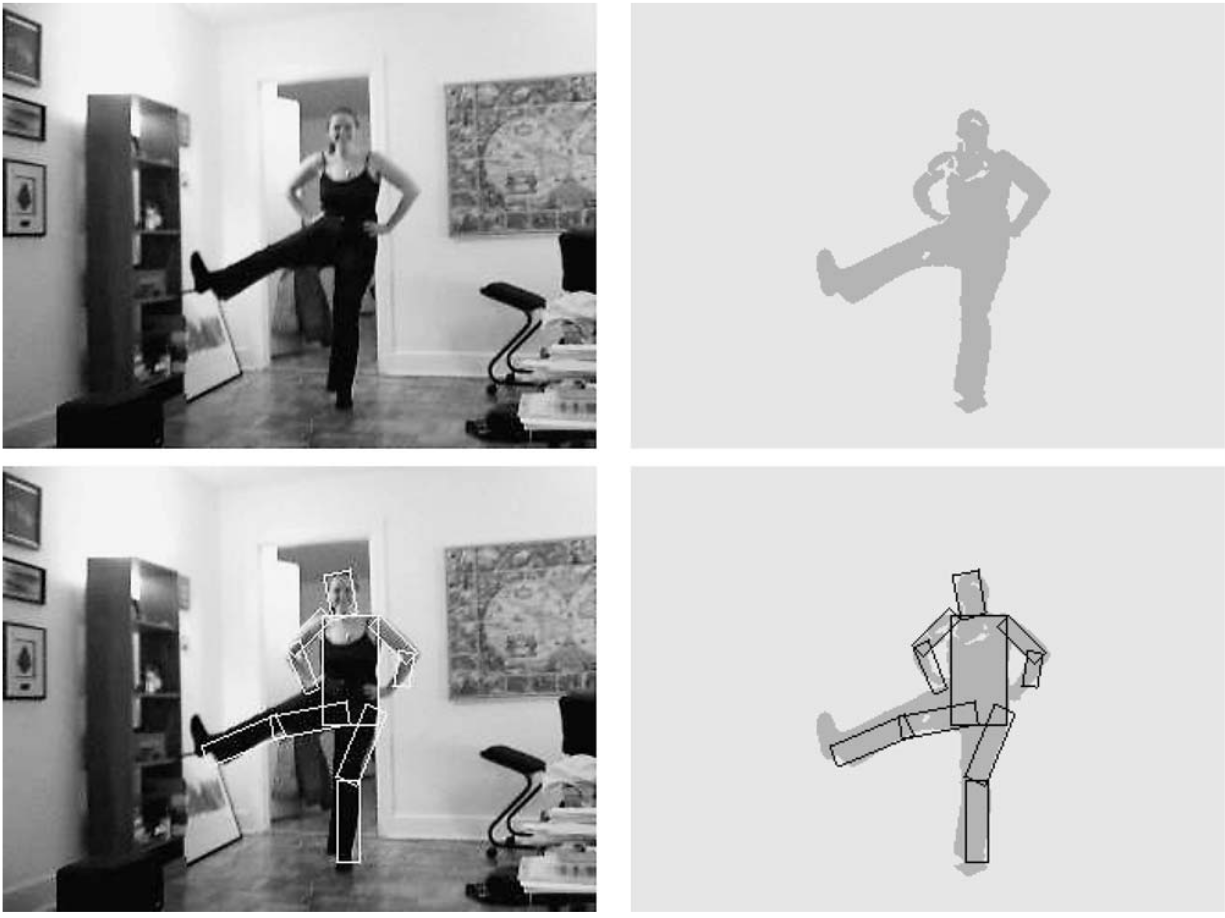
\includegraphics[width=.99\textwidth]{felzenszwalb-overview.png}
                \sourcefix{1}
            \end{figure}
        \end{column}
    \end{columns}
\end{myframe}

\begin{myframe}[Pose Estimation - Deep Methods]
    \begin{columns}[T]
        \begin{column}{.48\textwidth}
            \begin{itemize}
                %\vspace{25px}
                \item \textbf{Stacked hourglass network \footnotemark}
                  \begin{itemize}
                    \item Pooling, upsampling, skip-connections
                    \item 8 hourglasses back-to-back
                    \item Intermediate supervision
                    \item Residual modules~\footnotemark
                    \item Mean-squared Error
                    \item Refine result with each hourglass
                    \item Most state-of-the-art methods build on top
                  \end{itemize}
            \end{itemize}
        \end{column}
        \footnotetext[1]{\cite{newell_stacked_2016}}
        \footnotetext[2]{\cite{he_deep_2016}}
        \begin{column}{.48\textwidth}
            \begin{figure}
                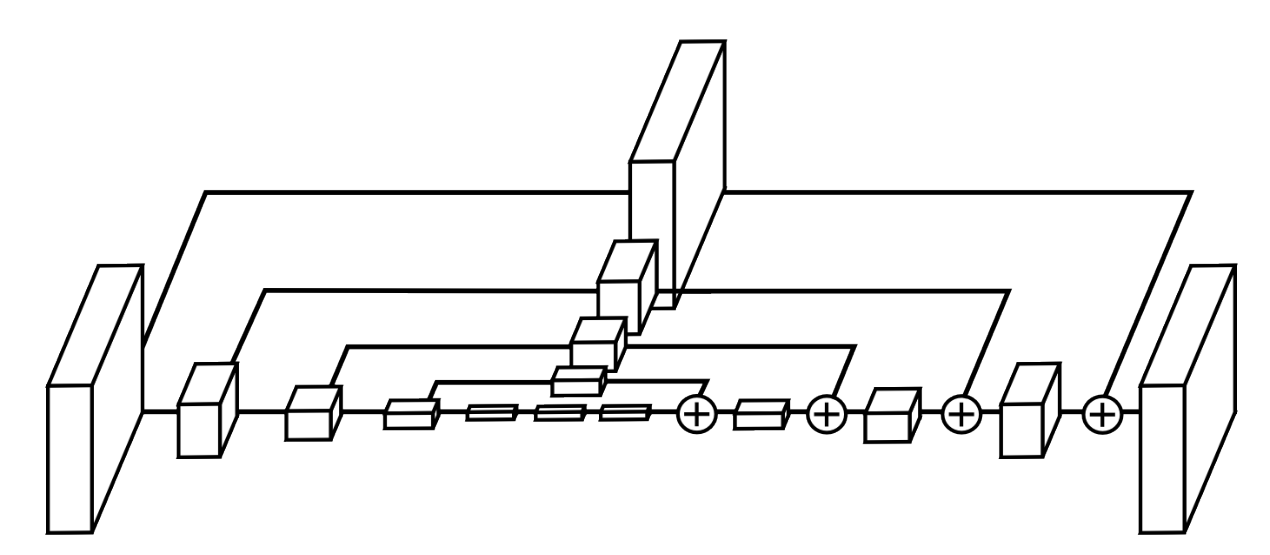
\includegraphics[width=.65\textwidth]{single-hourglass.png}
                \sourcefix{1}
            \end{figure}
            \begin{figure}
                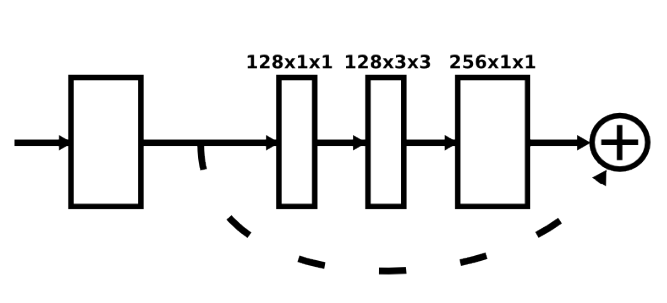
\includegraphics[width=.65\textwidth]{residualmodule.png}
                \sourcefix{2}
            \end{figure}
        \end{column}
    \end{columns}
    \begin{figure}
        \includegraphics[width=.65\textwidth]{stackedhourglass.png}
        \sourcefix{1}
    \end{figure}
\end{myframe}

\subsection{Video-based HAR}

\begin{myframe}[Video-based HAR - Shallow Methods]
	\begin{itemize}
		\item \textbf{Learning Realistic Human Actions from Movies \fcite{laptev_learning_2008}}
		\begin{itemize}
			\item Spatio-temporal extension of Harris corner detection
			\item Volume around interest points
			\begin{itemize}
                \item \textit{Histogram of oriented gradients (HoG)}
                \item \textit{Histogram of optical flow (HoF)}
				\item concatenation and normalization
			\end{itemize}
			\item Clustering into Bag-of-features
            \item Classification using Support Vector Machines (SVM)
		\end{itemize}
	\end{itemize}
	\begin{figure}
		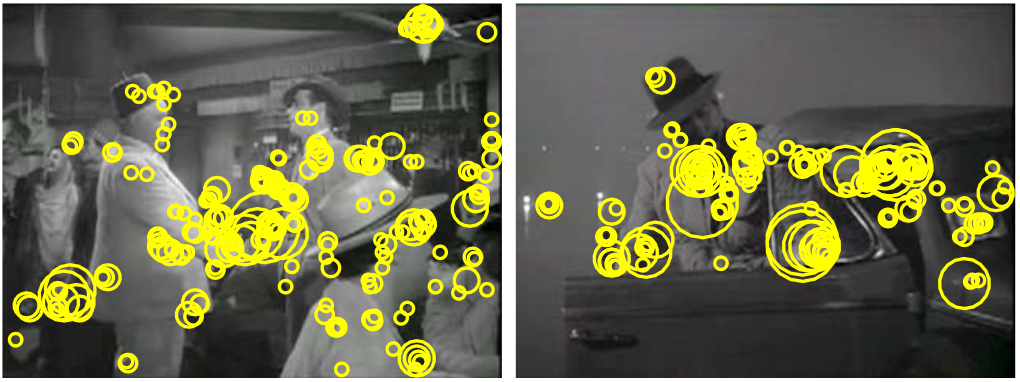
\includegraphics[width=.7\textwidth]{spacetimeinterestpoints.png}
        \caption{Left: Shaking hand, right: getting out of car.}
        \sourcefix{1}
	\end{figure}
\end{myframe}

\begin{myframe}[Video-based HAR - Deep Methods]
	\begin{itemize}
		\item \textbf{MiCT: Mixed Convolutional Tube \fcite{zhou_mict:_2018}}
		\begin{itemize}
			\item Third dimension $\Rightarrow$ temporal dimension
			\item Combining 2D and 3D convolutions more accurate than just 3D
			\item 4 MiCT blocks, followed by fully-connected layer
			\item State-of-the-art on HMDB51 for RGB-only methods
		\end{itemize}
	\end{itemize}
	\begin{figure}
		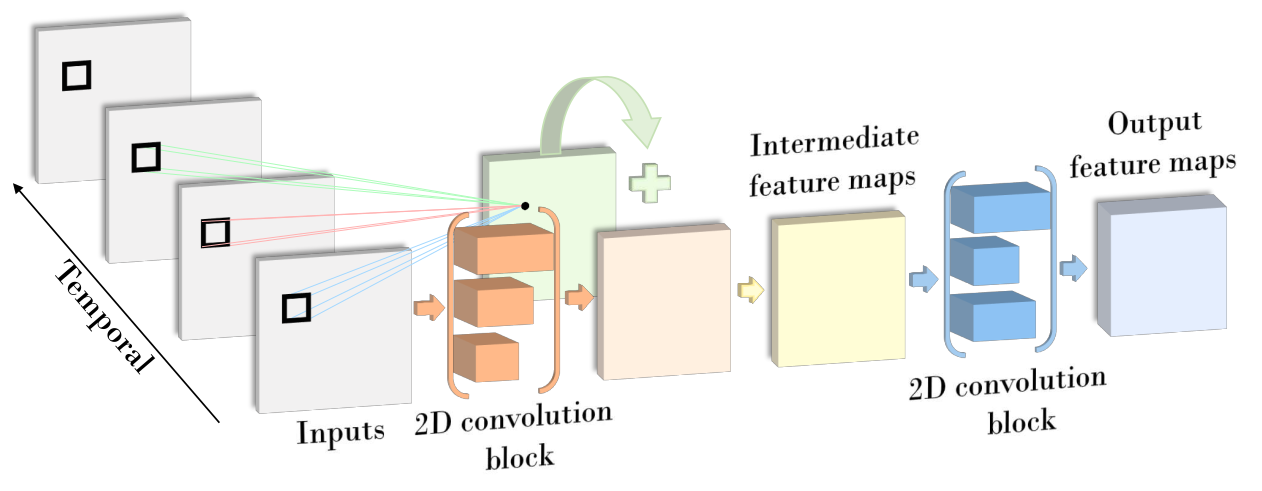
\includegraphics[width=.7\textwidth]{mict-block.png}
        \caption{Combining simple 2D convolutions with 3D convolutions.}
        \sourcefix{1}
	\end{figure}
\end{myframe}

\begin{myframe}[MiCT-Net]
	\begin{figure}
		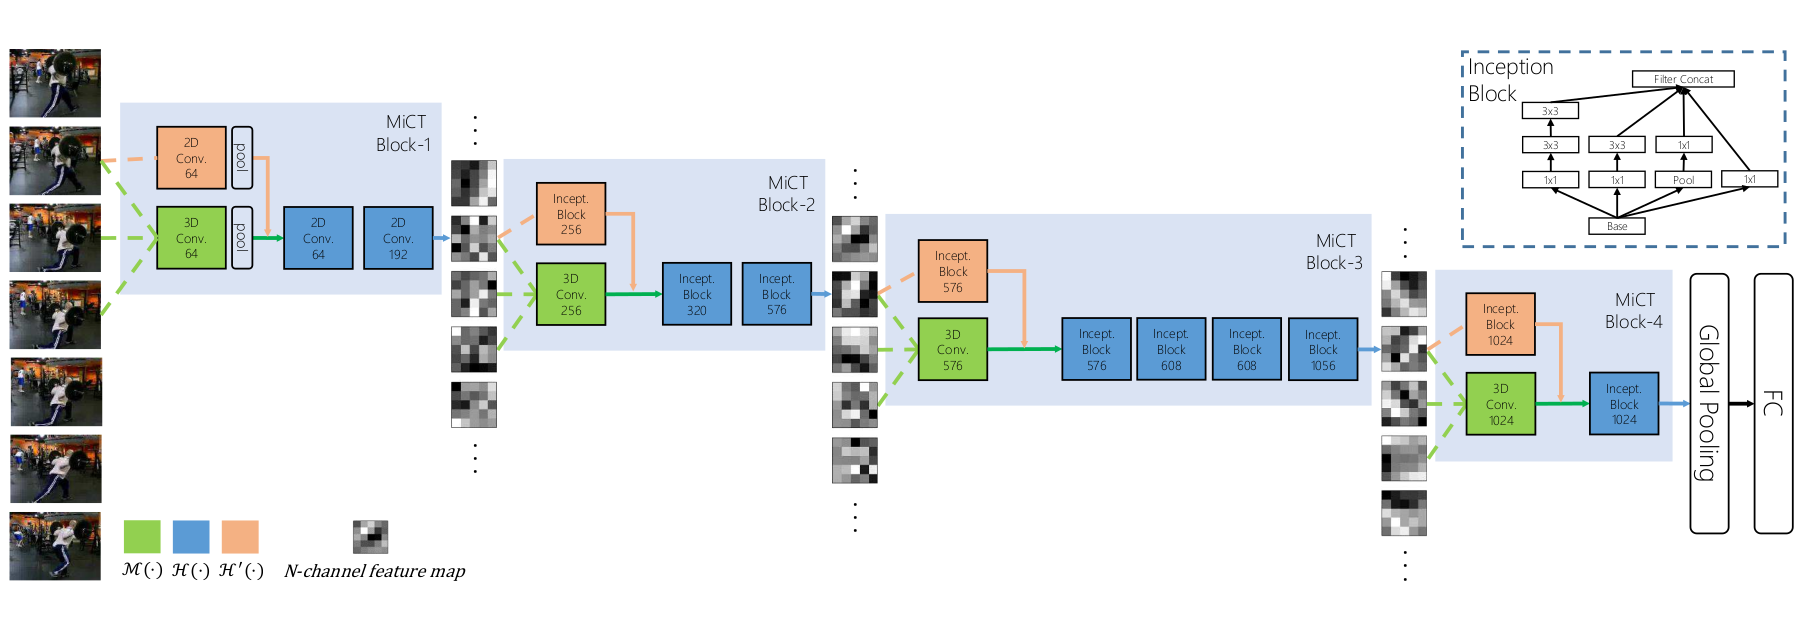
\includegraphics[width=.99\textwidth]{mict-full.png}
        \caption{Full architecture of MiCT-Net.}
        \source
	\end{figure}
    \footnotetext[1]{\cite{zhou_mict:_2018}}
\end{myframe}

\section{Method}

\begin{myframe}[Method - Joint methods]
	\begin{columns}[T]
	\begin{column}{.45\textwidth}
		\begin{itemize}
			\item \textbf{Multitask Deep HAR}\footnotemark
			\begin{itemize}
                \item Jointly train pose and action recognition
                \item Pre-train pose estimation part, then fine-tune end-to-end
				\item \textit{Soft-argmax}\footnotemark~makes end-to-end learning possible
			\end{itemize}
		\end{itemize}
        \begin{figure}
            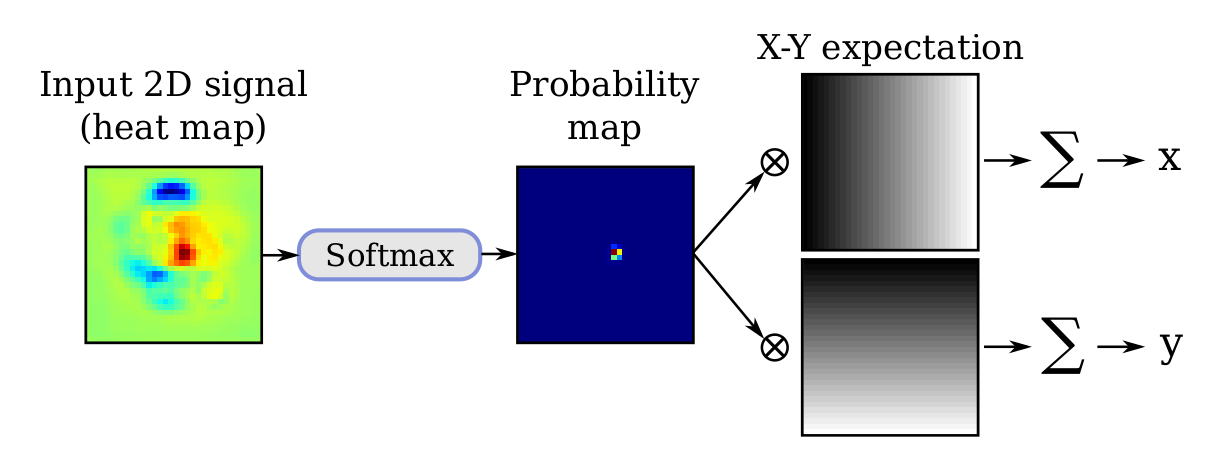
\includegraphics[width=0.99\textwidth]{softargmax.png}
            \sourcefix{1}
        \end{figure}
	\end{column}
    \footnotetext[1]{\cite{luvizon_2d/3d_2018}}
    \footnotetext[2]{\cite{luvizon_human_2017}}
	\begin{column}{.45\textwidth}
		\begin{figure}
			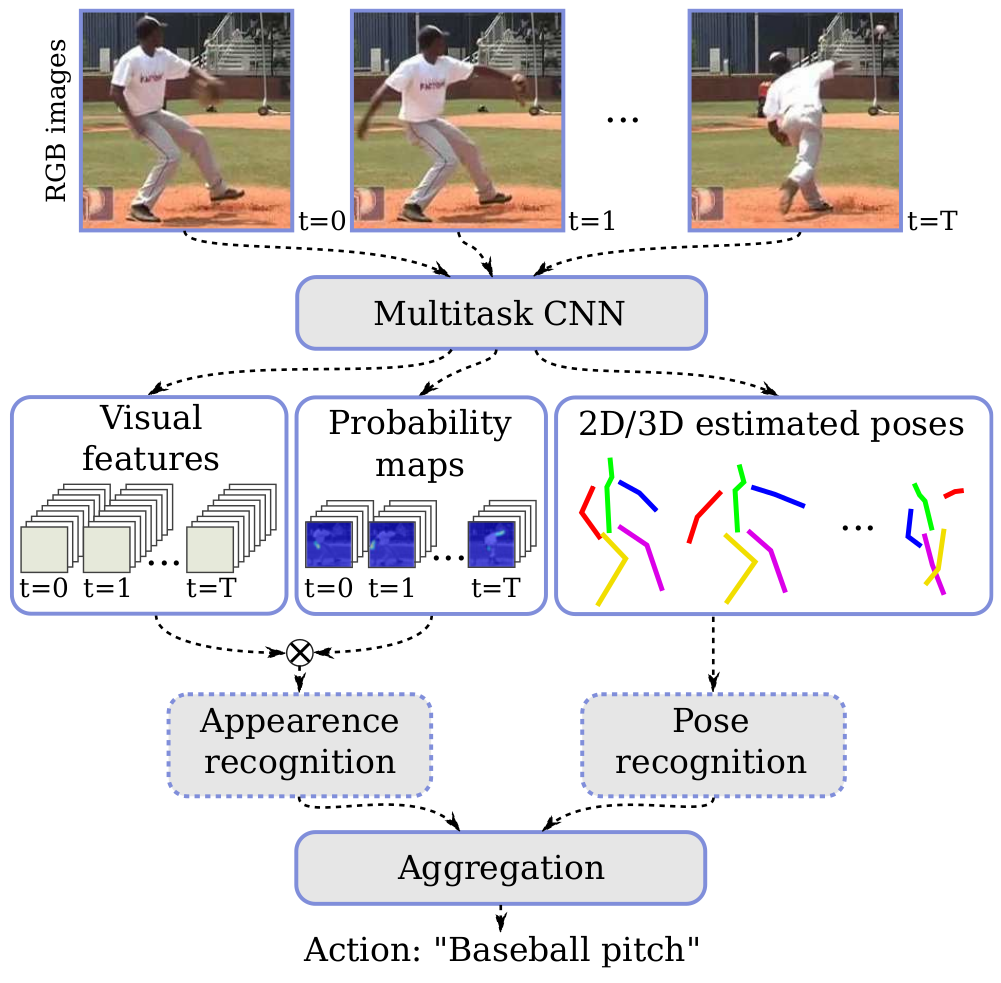
\includegraphics[width=.99\textwidth]{endtoend-concept.png}
            \sourcefix{1}
            %\caption{Complete network pipeline.}
		\end{figure}
	\end{column}
	\end{columns}
\end{myframe}

\begin{myframe}[Multitask Deep HAR - Architecture]
	\begin{columns}[T]
        \begin{column}{.45\textwidth}
            \begin{itemize}
                \item \textit{Multitask CNN}
                \begin{itemize}
                    \item Blocks similar to hourglasses
                    \item Refine prediction with each additional block
                    \item In addition to providing visual features and heatmaps:
                    \begin{itemize}
                        \item Coordinates from Soft-argmax
                        \item Join visibility vector using sigmoid
                    \end{itemize}
                \end{itemize}
            \end{itemize}
        \end{column}
        \begin{column}{.45\textwidth}
            \begin{figure}
                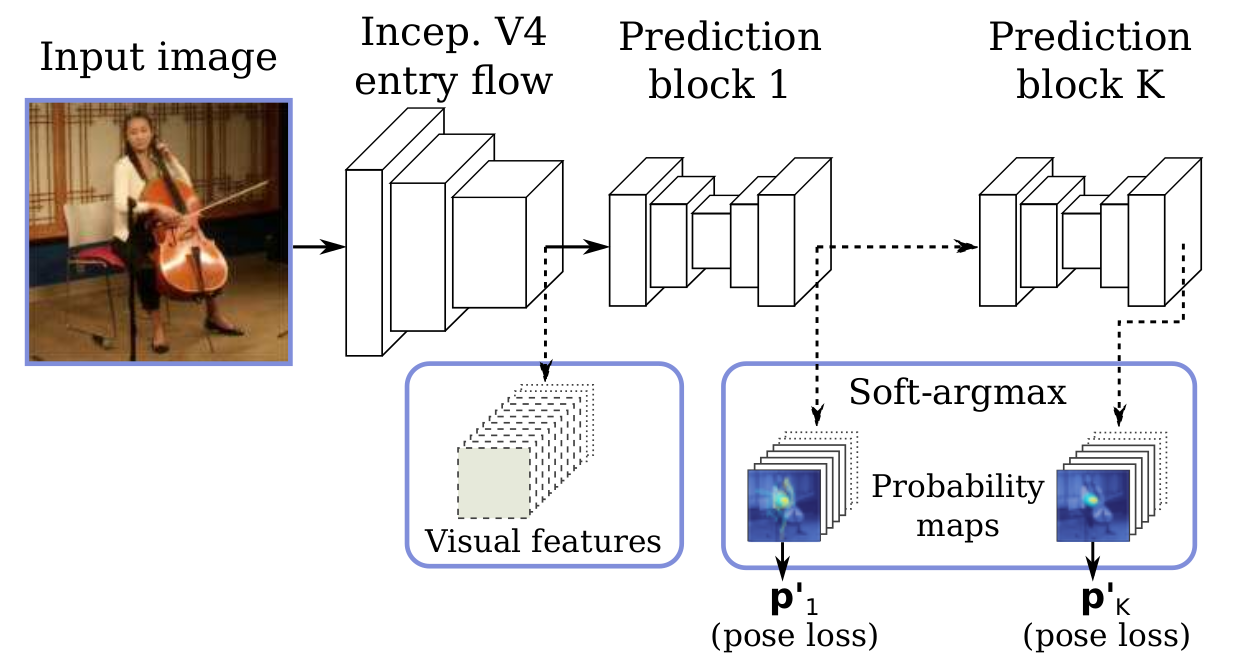
\includegraphics[width=.99\textwidth]{multitask-part.png}
                \sourcefix{1}
            \end{figure}
        \end{column}
	\end{columns}
    \footnotetext[1]{\cite{luvizon_2d/3d_2018}}
\end{myframe}

\begin{myframe}[Multitask Deep HAR - Architecture]
	\begin{columns}[T]
        \begin{column}{.45\textwidth}
            \begin{itemize}
                \item \textit{Pose recognition}
                \begin{itemize}
                    \item Arrange joint values over time in 2D matrix
                    \item Action heatmaps
                    \begin{itemize}
                        \item Through softmax: action probabilities
                    \end{itemize}
                    \item \textit{Max-min pooling}
                    \item Loss function $$L_p = \frac{1}{N_J}\sum_{n=1}^{N_J}(~ \lvert\lvert \hat{p}_n - p_n \rvert\rvert_1 ~+~ \lvert\lvert \hat{p}_n - p_n \rvert\rvert^2_2 ~ )$$
                \end{itemize}
            \end{itemize}
        \end{column}
        \begin{column}{.45\textwidth}
            \begin{figure}
                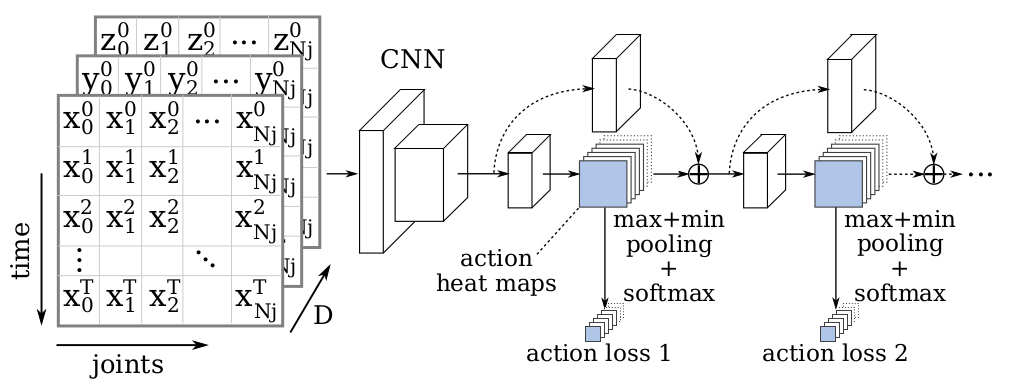
\includegraphics[width=.99\textwidth]{jointsovertime.png}
                \sourcefix{1}
            \end{figure}
        \end{column}
	\end{columns}
    \footnotetext[1]{\cite{luvizon_2d/3d_2018}}
\end{myframe}

\begin{myframe}[Multitask Deep HAR - Architecture]
	\begin{columns}[T]
        \begin{column}{.45\textwidth}
            \begin{itemize}
                \item \textit{Appearance recognition}
                \begin{itemize}
                    \item Combination of visual features and joint positions
                    \item Then: Identical architecture to pose recognition part
                \end{itemize}
                \item \textit{Aggregation}
                \begin{itemize}
                    \item Combine pose recognition and appearance recognition for final result
                    \item \textit{Categorical cross-entropy}
                \end{itemize}
            \end{itemize}
        \end{column}
        \begin{column}{.45\textwidth}
            \begin{figure}
                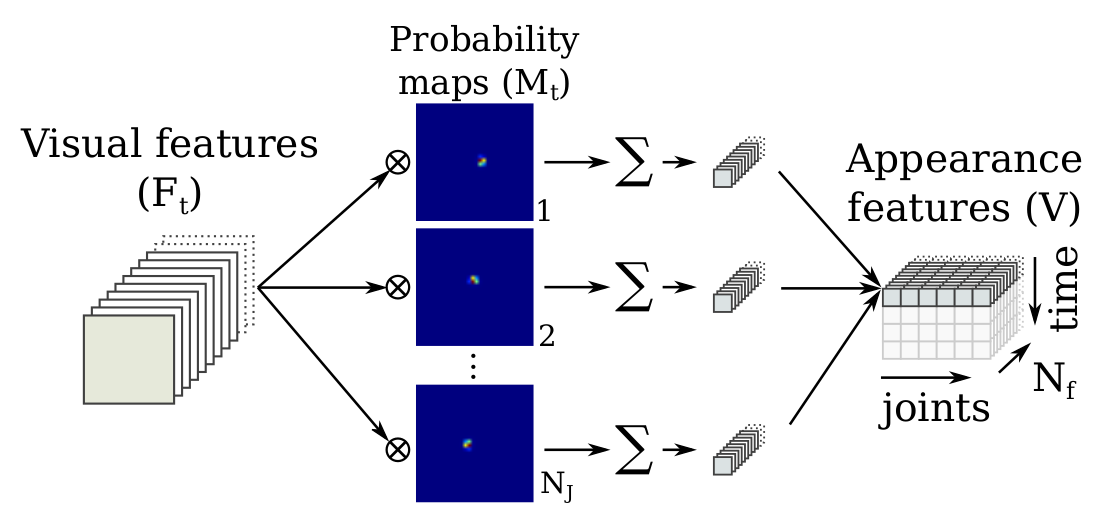
\includegraphics[width=.99\textwidth]{appearance-features.png}
                \sourcefix{1}
            \end{figure}
        \end{column}
	\end{columns}
    \footnotetext[1]{\cite{luvizon_2d/3d_2018}}
\end{myframe}

\begin{myframe}[Method]
    \begin{itemize}
        \item Reimplementation in PyTorch \fcite{paszke_automatic_2017}
        \begin{itemize}
            \item Evaluate against HMDB \fcite{kuehne_hmdb:_2011}
        \end{itemize}
        \item Experimentation
        \begin{itemize}
            %\item Better incorporation of temporal dimension \fcite{pavllo_3d_2019}
            \item Compare with state-of-the-art methods not using pose \fcite{zhou_mict:_2018}
            \item Different representation of temporal information (next slide)
            \item Combined loss function of pose and action for \emph{real} end-to-end training
        \end{itemize}
    \end{itemize}
\end{myframe}

\begin{myframe}[Method]
    \begin{figure}
        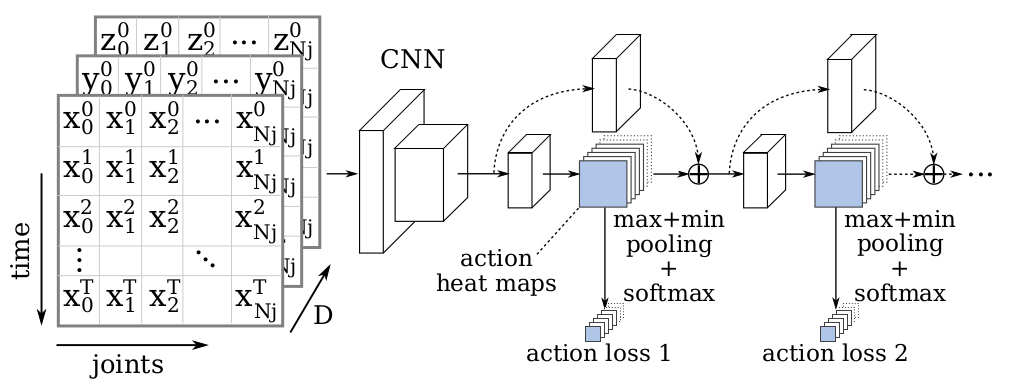
\includegraphics[width=.65\textwidth]{jointsovertime.png}
        \caption{Approach used by \footnotemark. Convolution over all sensors at once. \sourcefix{1}}
    \end{figure}
    \begin{figure}
        \includegraphics[width=.65\textwidth]{sensor-time.png}
        \caption{Impression of pixel coordinates of joints over time \source}
    \end{figure}
    \footnotetext[1]{\cite{luvizon_2d/3d_2018}}
    \footnotetext[2]{\url{https://avtech.com/articles/wp-content/uploads/2015/06/Intro.-Pic.png}}
\end{myframe}

\section{Datasets}
% also: metrics?
% \begin{myframe}[2D / 3D pose datasets]
%   \begin{itemize}
%       \item \textbf{2D}
%       \begin{itemize}
%           \item MPII \fcite{andriluka_2d_2014}
%           \item LSP \fcite{johnson_clustered_2010}\fcite{johnson_learning_2011}
%       \end{itemize}
%       \item \textbf{3D}
%       \begin{itemize}
%           \item Human 3.6M \fcite{ionescu_human3.6m:_2014}
%       \end{itemize}
%   \end{itemize}
% \end{myframe}

\begin{myframe}[2D Pose Datasets]
  \begin{columns}[T]
      \begin{column}{.48\textwidth}
          \begin{itemize}
              \item \textbf{MPII Human Pose\footnotemark}
              \begin{itemize}
                  \item 40,000 annotated images
                  \item Single and multi person
                  \item Over 401 different activities
              \end{itemize}
          \end{itemize}
      \end{column}
      \footnotetext[1]{\cite{andriluka_2d_2014}}
      \begin{column}{.48\textwidth}
          \begin{figure}
              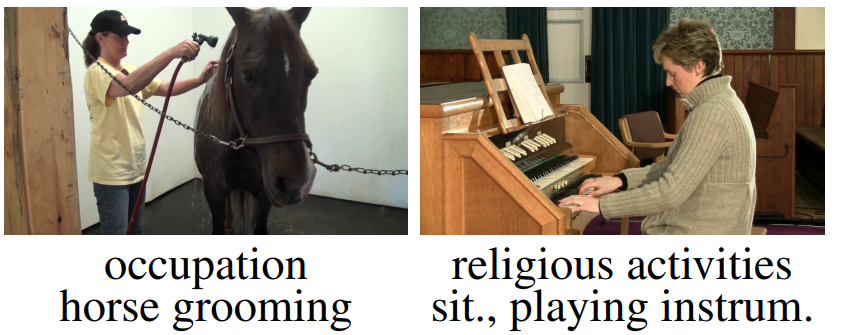
\includegraphics[width=0.99\textwidth]{mpii.png}
              \sourcefix{1}
          \end{figure}
      \end{column}
  \end{columns}
\end{myframe}

% \begin{myframe}[3D Pose Datasets]
%   \begin{columns}[T]
%       \begin{column}{.48\textwidth}
%           \vspace{50px}
%           \begin{itemize}
%               \item \textbf{Human3.6m\footnotemark}
%               \begin{itemize}
%                   \item 3,600,000 annotated images
%                   \item Annotated using motion capturing system
%                   \item 11 male and female actors recreate daily situations
%                   \item 17 different scenarios
%               \end{itemize}
%           \end{itemize}
%       \end{column}
%       \footnotetext[1]{\cite{ionescu_human3.6m:_2014}}
%       \begin{column}{.48\textwidth}
%           \begin{figure}
%               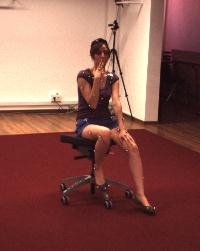
\includegraphics[width=0.48\textwidth]{human-01.jpg}
%               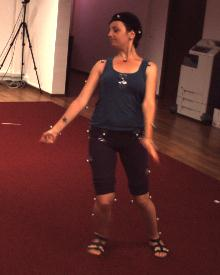
\includegraphics[width=0.48\textwidth]{human-02.jpg}
%               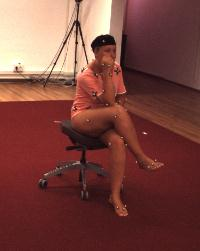
\includegraphics[width=0.48\textwidth]{human-03.jpg}
%               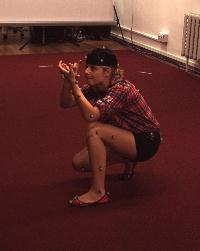
\includegraphics[width=0.48\textwidth]{human-04.jpg}
%               \source
%           \end{figure}
%       \end{column}
%   \end{columns}
%   \footnotetext[2]{\url{http://vision.imar.ro/human3.6m/description.php}}
% \end{myframe}

% \begin{myframe}[2D HAR datasets]
%   \begin{itemize}
%       \item Penn Action \fcite{zhang_actemes_2013}
%       \item HMDB51 \fcite{kuehne_hmdb:_2011}
%       \item Kinetics \fcite{kay_kinetics_2017}
%   \end{itemize}
% \end{myframe}

\begin{myframe}[Action Recognition Datasets]
  \begin{columns}[T]
      \begin{column}{.48\textwidth}
          \vspace{20px}
          \begin{itemize}
              \item \textbf{Penn Action\footnotemark}
              \begin{itemize}
                  \item 2,400 video clips of 15 actions
                  \item Very limited number of actions (mainly sport)
              \end{itemize}
          \end{itemize}
      \end{column}
      \footnotetext[1]{\cite{zhang_actemes_2013}}
      \begin{column}{.48\textwidth}
          \begin{figure}
              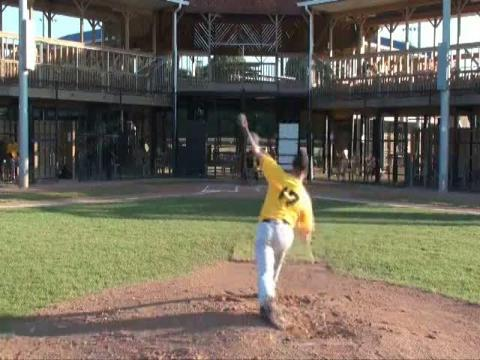
\includegraphics[height=45px]{pa-01.jpg}
              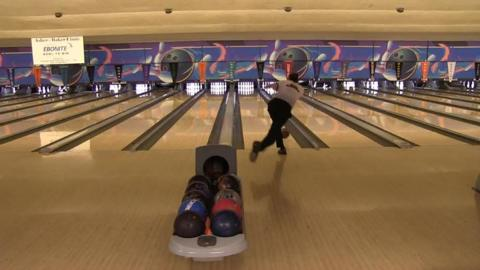
\includegraphics[height=45px]{pa-02.jpg}
              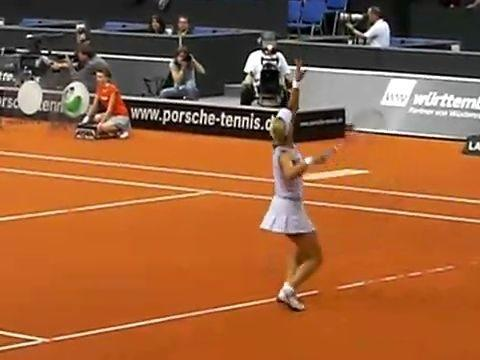
\includegraphics[height=45px]{pa-03.jpg}
              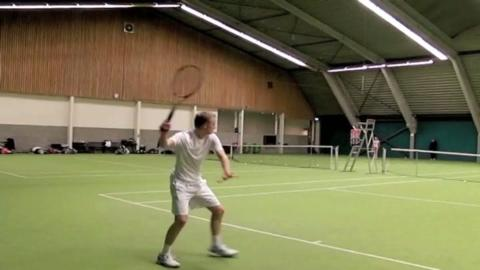
\includegraphics[height=45px]{pa-04.jpg}
              \source
          \end{figure}
      \end{column}
  \end{columns}
  \footnotetext[2]{\url{https://upenn.app.box.com/v/PennAction}}
\end{myframe}

\begin{myframe}[Action Recognition Datasets]
  \begin{columns}[T]
      \begin{column}{.48\textwidth}
          \begin{itemize}
              \item \textbf{HMDB51\footnotemark}
              \begin{itemize}
                  \item 6,800 video clips of 51 actions
                  \item Video clips from youtube
                  \item At least 101 clips per action category
              \end{itemize}
          \end{itemize}
      \end{column}
      \footnotetext[1]{\cite{kuehne_hmdb:_2011}}
      \begin{column}{.48\textwidth}
          \begin{figure}
              \includegraphics[height=.55\textheight]{hmdb-example.png}
              \source
          \end{figure}
      \end{column}
  \end{columns}
  \footnotetext[2]{\url{http://serre-lab.clps.brown.edu/wp-content/uploads/2012/08/HMDB_snapshot1.png}}
\end{myframe}

\begin{myframe}[Action Recognition Datasets]
  \begin{columns}[T]
      \begin{column}{.48\textwidth}
          \begin{itemize}
              \item \textbf{J-HMDB\footnotemark}
              \begin{itemize}
                  \item Fully-annotated subset of HMDB
                  \begin{itemize}
                      \item 2D pose, person segmentation maps etc.
                  \end{itemize}
                  \item 928 clips of 21 actions
                  \item Can be used for end-to-end training
              \end{itemize}
          \end{itemize}
      \end{column}
      \footnotetext[1]{\cite{jhuang_towards_2013}}
      \begin{column}{.48\textwidth}
          \begin{figure}
              \includegraphics[height=.55\textheight]{jhmdb.png}
              \centering
              \source
          \end{figure}
      \end{column}
  \end{columns}
  \footnotetext[2]{\url{http://jhmdb.is.tue.mpg.de/puppet_tool}}
\end{myframe}

\section{Conclusion}
\begin{myframe}[Conclusion]
    \begin{itemize}
        \item Promising results combining pose and action recognition
        \item But: Barely any publications in the past year
        \item Much experimentation possible
        \item Future work:
        \begin{itemize}
            \item Multi-person end-to-end pipeline
            \item Bigger pose-annotated \emph{in-the-wild} action datasets necessary
        \end{itemize}
    \end{itemize}
\end{myframe}

\begin{myframe}[Thank you]
    \centering \Large
    \emph{Thank you for your time!}
\end{myframe}

\end{document}

